% Design review: IoT-Based Cold Chain Monitoring for Vaccine Storage Units
% 04-645 A Internet of Things, CMU Africa, Fall 2026
% Compile with pdfLaTeX (Overleaf: upload this folder, including figures/).
% Red \note{} blocks are instructions for the team: delete them before submitting.

\documentclass[conference,12pt]{IEEEtran}

\IfFileExists{lmodern.sty}{\usepackage{lmodern}}{\usepackage{mathptmx}}
\usepackage[T1]{fontenc}
\usepackage{textcomp}
\usepackage{graphicx}
\usepackage{array}
\usepackage{booktabs}
\usepackage{xcolor}
\usepackage{tikz}
\usetikzlibrary{positioning,arrows.meta,shapes.geometric,fit,backgrounds}
\usepackage{forest}
\usepackage{dirtree}
\usepackage{balance}
\usepackage{url}
\usepackage{cite}

\definecolor{noteRed}{RGB}{200,0,0}
\definecolor{edgeC}{RGB}{226,239,218}
\definecolor{netC}{RGB}{222,235,247}
\definecolor{cloudC}{RGB}{255,242,204}
\definecolor{appC}{RGB}{237,226,246}

% Red instruction to the team. Delete every \note before submitting.
\newcommand{\note}[1]{%
  \par\medskip
  {\leftskip=1.2em\rightskip=1.2em\small\itshape\color{noteRed}#1\par}%
  \medskip}
\newcommand{\degC}{\,\textdegree{}C}

\begin{document}

\title{IoT-Based Cold Chain Monitoring for\\ Vaccine Storage Units: Design Review}

\author{%
\IEEEauthorblockN{Putshu Lunghe Samuel}
\IEEEauthorblockA{Andrew ID: plunghe}
\and
\IEEEauthorblockN{Yves Dominique Gatoni}
\IEEEauthorblockA{Andrew ID: ygatoni}
\and
\IEEEauthorblockA{Carnegie Mellon University Africa, Kigali, Rwanda\\
04-645 A: Internet of Things, Fall 2026}}

\maketitle

\note{Before you submit: (1) compile on Overleaf and check the PDF is 5 pages or fewer and the last
page's columns are balanced; (2) check every status in Table~II is true today; (3) delete all red
notes. If the report is over 5 pages, first shrink Fig.~4 to 0.8 of the page width, then shorten
Section~III.}

\section{Introduction}

Vaccines must be stored between +2\degC{} and +8\degC{} \cite{who2006}. In a health centre they
sit in an ordinary fridge or cool box, and the temperature is often checked by hand only twice a
day. A power cut or a door left open can push the fridge out of range for hours before anyone
notices, and afterwards nobody knows how long it lasted or which stock is affected.

Our system turns one storage unit into a monitored Web Thing. A node on the fridge measures the
internal temperature, the room temperature and humidity, the state of the door, and whether the
12~V supply that powers the cooling is present. When the unit is out of range, the door stays open
too long, or the power is lost, the node sounds a buzzer, lights a red LED and shows the cause on a
display. The cloud sends an SMS to the supervisor, who can check the unit from any browser through
its W3C Thing Description \cite{wot-td}. The node keeps a running total of the time spent out of
range, with a record of each excursion (start, end, minimum and maximum), so that affected stock
can be identified. As an extension, a keypad and a solenoid lock control who opens the fridge.

Since the proposal, we have finished the edge firmware, the back end and the dashboard, and
tested them together with a simulated node. This review describes the design and the hardware we
are now building, and the progress so far.

\section{Design}

\subsection{Project Scenario}

Fig.~\ref{fig:scenario} shows the scenario. The node sits on the vaccine fridge in the store of a
health centre and connects to the building's Wi-Fi. It sends its data to a cloud MQTT broker. Our
back end turns these messages into a Web Thing, stores them and sends SMS alerts. The supervisor
uses a web dashboard, and a nurse can unlock the fridge with a PIN or with a QR code on the door.

\begin{figure}[!t]
\centering
% Drawn at its final size (no scaling), so lines and arrowheads stay thin.
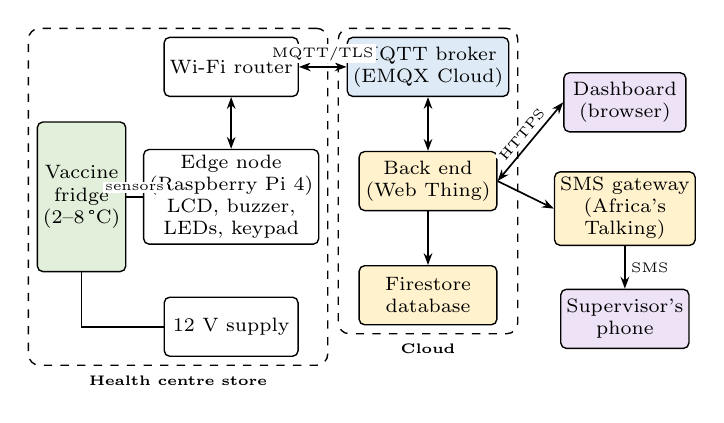
\begin{tikzpicture}[font=\scriptsize,
  box/.style={draw, line width=0.5pt, rounded corners=2pt, align=center, inner sep=2pt,
              minimum height=0.75cm},
  line/.style={line width=0.6pt},
  link/.style={line width=0.6pt, -{Stealth[length=1.5mm, width=1.1mm]}},
  both/.style={line width=0.6pt, {Stealth[length=1.5mm, width=1.1mm]}-{Stealth[length=1.5mm, width=1.1mm]}},
  lbl/.style={font=\tiny, fill=white, inner sep=1pt}]
  % ---- health centre store (left)
  \node[box, fill=edgeC, minimum width=1.0cm, minimum height=1.9cm] (fridge) at (0.6,-0.2)
    {Vaccine\\fridge\\(2--8\degC)};
  \node[box, fill=white, minimum width=1.7cm] (pinode) at (2.5,-0.2)
    {Edge node\\(Raspberry Pi 4)\\LCD, buzzer,\\LEDs, keypad};
  \node[box, fill=white, minimum width=1.7cm] (router) at (2.5,1.45) {Wi-Fi router};
  \node[box, fill=white, minimum width=1.7cm] (psu) at (2.5,-1.85) {12 V supply};
  \draw[line] (pinode.west) -- node[lbl, above=1pt]{sensors} (fridge.east);
  \draw[line] (psu.west) -| (fridge.south);
  \draw[both] (pinode) -- (router);
  \begin{scope}[on background layer]
    \node[draw, dashed, line width=0.5pt, rounded corners, fit=(fridge)(pinode)(psu)(router),
      inner sep=3pt] (site) {};
  \end{scope}
  \node[font=\tiny\bfseries, anchor=north] at (site.south) {Health centre store};
  % ---- cloud (middle)
  \node[box, fill=netC, minimum width=1.75cm] (broker) at (5.0,1.45) {MQTT broker\\(EMQX Cloud)};
  \node[box, fill=cloudC, minimum width=1.75cm] (backend) at (5.0,0.0) {Back end\\(Web Thing)};
  \node[box, fill=cloudC, minimum width=1.75cm] (db) at (5.0,-1.45) {Firestore\\database};
  \draw[both] (router) -- node[lbl, above=1pt]{MQTT/TLS} (broker);
  \draw[both] (broker) -- (backend);
  \draw[link] (backend) -- (db);
  \begin{scope}[on background layer]
    \node[draw, dashed, line width=0.5pt, rounded corners, fit=(broker)(backend)(db),
      inner sep=3pt] (cloud) {};
  \end{scope}
  \node[font=\tiny\bfseries, anchor=north] at (cloud.south) {Cloud};
  % ---- supervisor (right)
  \node[box, fill=appC, minimum width=1.55cm] (dash) at (7.5,1.0) {Dashboard\\(browser)};
  \node[box, fill=cloudC, minimum width=1.55cm] (sms) at (7.5,-0.35) {SMS gateway\\(Africa's\\Talking)};
  \node[box, fill=appC, minimum width=1.55cm] (phone) at (7.5,-1.75) {Supervisor's\\phone};
  \draw[both] (backend.east) -- node[lbl, above=1pt, sloped]{HTTPS} (dash.west);
  \draw[link] (backend.east) -- (sms.west);
  \draw[link] (sms) -- node[lbl, right=1pt]{SMS} (phone);
\end{tikzpicture}
\caption{Project scenario: one monitored vaccine fridge in a health centre store, connected
through the building's Wi-Fi to the cloud. The back end serves the dashboard and sends SMS
alerts to the supervisor's phone.}
\label{fig:scenario}
\end{figure}

\note{The manual asks for an original image of the scenario. Fig.~1 is drawn by us in TikZ. If you
prefer, replace it with a photo or a drawing of your own setup.}

\subsection{Major Components and Their Justification}

Table~\ref{tab:components} lists the four layers, the choice we made in each, and why.

\emph{Edge.} A Raspberry Pi~4 runs all the alarm logic itself, so the local alarm keeps working
when the Internet is down. A DS18B20 waterproof probe inside the fridge gives the internal
temperature; a DHT22 outside gives the room temperature and humidity, so we can tell a failing
fridge from a hot room. A magnetic reed switch senses the door. A 10~k$\Omega$/2.7~k$\Omega$
divider brings the 12~V supply down to 2.55~V on a GPIO input, which tells the node whether power
is present. The outputs are a passive buzzer driven by a transistor, red and green LEDs, and a
16$\times$2 LCD. The LCD runs on 5~V, so a BSS138 level shifter protects the Pi's 3.3~V I2C pins.
For the extension, a 4$\times$4 keypad takes a PIN and a solenoid lock secures the door.

\emph{Gateway.} We do not use a separate gateway. The Pi has Wi-Fi and enough power to run TLS,
and a health centre usually has Wi-Fi, so the node talks to the cloud directly. This removes one
device that could fail.

\emph{Connectivity.} The node uses MQTT \cite{mqtt5} over TLS on port 8883. MQTT is light, keeps
one connection open for both directions, and its ``last will'' message tells the cloud at once
when the node goes offline. When the connection is lost, the node stores its messages in a local
database and sends them in order later.

\emph{Application.} A Node.js back end subscribes to the broker. It serves the Thing Description
and its properties, actions and events over HTTP, stores data in Firebase Firestore, and sends SMS
through Africa's Talking, which works in Rwanda and reaches any phone. Every alert also goes to a
Telegram bot as a backup channel (Section~\ref{sec:discussion}). A React dashboard shows the
live status, a temperature chart with the safe band, the excursions and simple analytics.

\begin{table*}[!t]
\caption{Major components and the reasons for each choice}
\label{tab:components}
\centering
\footnotesize
\renewcommand{\arraystretch}{1.15}
\begin{tabular}{@{}p{2.0cm}p{5.2cm}p{8.6cm}@{}}
\toprule
\textbf{Layer} & \textbf{Choice} & \textbf{Justification} \\
\midrule
Edge &
Raspberry Pi 4 Model B; Python application &
Runs the alarm logic locally (works offline); built-in Wi-Fi; enough memory for TLS and an
offline message queue; available in the lab. \\
Sensors &
DS18B20 probe (inside); DHT22 (outside); MC-38 reed switch (door); 12 V voltage divider (power) &
Waterproof probe with $\pm$0.5\degC{} accuracy; ambient reading separates a fridge fault from a
hot room; reed switch needs no power; divider is cheap and keeps the GPIO below 3.3~V. \\
Actuators &
Passive buzzer; red and green LEDs; 16$\times$2 I2C LCD; solenoid lock with relay module &
Local alarm that needs no network; LCD shows the cause; the relay keeps the lock current away from
the Pi (no logic-level MOSFET was available locally). \\
Gateway &
None: the node connects directly &
The Pi has Wi-Fi and runs TLS itself; one less device to fail. \\
Connectivity &
MQTT over TLS (port 8883) to EMQX Cloud Serverless &
Light publish--subscribe protocol, two-way, last-will message for offline detection; free plan
with a trusted TLS certificate. \\
Cloud and WoT &
Node.js back end on Railway; W3C Thing Description 1.1; Firestore; Africa's Talking SMS;
Telegram bot &
Standard Web Thing interface for any client; managed database with real-time listeners; SMS
reaches basic phones in Rwanda; Telegram is a free, reliable backup for the alerts. \\
Application &
React dashboard and QR unlock page &
Works on a laptop and a phone; supervisors sign in; the QR page links each unlock to a person. \\
\bottomrule
\end{tabular}
\end{table*}

\subsection{Resource Decision Tree}

We designed the resources the same way as in our homework: first the hierarchy of URLs, then the
interactions of each Thing. Fig.~\ref{fig:tree-full} shows the hierarchical resource tree of the
full design. A real deployment has many health centres, each with several storage units. Each unit
groups its resources by the hardware they come from: sensors, door, power, alarm state and
actuators. The dashed circles are resources of the full design that we leave out of the prototype:
more than one facility and unit, the lock state, the backup battery level and the location.

Fig.~\ref{fig:tree-reduced} shows the reduced version that we implement: one Thing,
\emph{cold-unit-01}, for one fridge. Each resource is marked with its kind of interaction and the
operation it supports. The thresholds are both a writable property and an action, because the
brief asks for both kinds of interaction.

\begin{figure*}[!t]
\centering
\begin{forest}
  for tree={
    grow'=0, circle, draw, minimum size=2.4mm, inner sep=0pt, fill=gray!25,
    l sep=16mm, s sep=1mm, anchor=center,
    edge={gray, -{Stealth[length=1.1mm, width=0.9mm]}}},
  n/.style={label={[font=\scriptsize, inner sep=1pt]above:#1}},
  leaf/.style={fill=white, label={[font=\scriptsize, inner sep=1pt]right:#1}},
  full/.style={dashed, draw=gray},
  fullleaf/.style={fill=white, dashed, draw=gray,
    label={[font=\scriptsize\itshape, text=gray, inner sep=1pt]right:#1}},
[, n={\textbf{www.coldchain.rw/facilities}}, fill=blue!20
  [, n=facility1, fill=orange!35
    [, n=units
      [, n=unit1, fill=green!35
        [, n=sensors
          [, leaf=internalTemperature]
          [, leaf=ambientTemperature]
          [, leaf=humidity]
        ]
        [, n=door
          [, leaf=doorOpen]
          [, fullleaf=lockState]
        ]
        [, n=power
          [, leaf=mainsPower]
          [, fullleaf=batteryLevel]
        ]
        [, n=alarm
          [, leaf=status]
          [, leaf=outOfRangeSeconds]
          [, leaf=thresholds]
        ]
        [, n=actuators
          [, leaf=buzzer]
          [, leaf=redLed]
          [, leaf=greenLed]
          [, leaf=lcd]
          [, leaf=lock]
        ]
        [, n=gps, full
          [, fullleaf=latitude]
          [, fullleaf=longitude]
        ]
      ]
      [, n=unit2, full, fill=green!15
        [, fullleaf={same structure as unit1}]
      ]
    ]
  ]
  [, n=facility2, full, fill=orange!15
    [, fullleaf={same structure as facility1}]
  ]
]
\end{forest}
\caption{Hierarchical resource tree of the full design: facilities, then their storage units,
then the resources of each unit grouped by hardware. Dashed circles belong to the full design
only; the prototype implements one unit.}
\label{fig:tree-full}
\end{figure*}

\begin{figure}[!t]
\centering
\begin{minipage}{\columnwidth}
\scriptsize
\dirtree{%
.1 \textbf{COLD CHAIN UNIT} (/things/cold-unit-01).
.2 \texttt{status}: Property; Read.
.2 \texttt{outOfRangeSeconds}: Property; Read.
.2 \texttt{thresholds}: Property; Read/Write.
.2 sensors.
.3 \texttt{internalTemperature}: Property; Read.
.3 \texttt{ambientTemperature}: Property; Read.
.3 \texttt{humidity}: Property; Read.
.3 \texttt{doorOpen}: Property; Read.
.3 \texttt{mainsPower}: Property; Read.
.2 Actions.
.3 \texttt{acknowledgeAlarm}: Invoke.
.3 \texttt{setThresholds}: Invoke.
.3 \texttt{unlockDoor}: Invoke.
.2 Events.
.3 \texttt{OUT\_OF\_RANGE\_HIGH}, \texttt{\_LOW}: Subscribe.
.3 \texttt{BACK\_IN\_RANGE}: Subscribe.
.3 \texttt{DOOR\_OPEN\_TOO\_LONG}, \texttt{DOOR\_CLOSED}: Subscribe.
.3 \texttt{POWER\_LOST}, \texttt{POWER\_RESTORED}: Subscribe.
.3 \texttt{SENSOR\_FAULT}, \texttt{SENSOR\_RESTORED}: Subscribe.
.3 \texttt{ALARM\_ACKNOWLEDGED}: Subscribe.
.3 \texttt{ACCESS\_GRANTED}, \texttt{ACCESS\_DENIED}: Subscribe.
}
\end{minipage}
\caption{Resource tree of the reduced version we implement: one Thing for one fridge, with
8 properties, 3 actions and 12 event types. In the Thing Description each property is served at
/things/cold-unit-01/properties/\{name\}.}
\label{fig:tree-reduced}
\end{figure}

\subsection{Hardware of the Reduced Version}

Fig.~\ref{fig:fritzing} shows the Fritzing model of the circuit we build on the breadboard. The
top rails carry 3.3~V and the bottom rails 5~V; both share ground with the Pi. The probe has a
4.7~k$\Omega$ pull-up on its 1-Wire line. The 12~V sense input has a 1~k$\Omega$ series resistor,
a 100~nF filter and a Schottky clamp to 3.3~V, in case the adapter gives more than 12~V.

Safety drove three choices. First, the 120~W Peltier cooling kit draws about 8--10~A at 12~V.
This current flows only from a certified 12~V, 30~A supply through a 15~A fuse and a 30~A car
relay to the Peltier; the W1209 thermostat switches only the relay's coil, because its own relay
is rated for about 10~A. It never passes through the breadboard or the Pi; only the divider's 1~mA does.
Nobody touches 230~V. Second, the lock has its own adapter and is switched by the relay contacts.
Third, the lock must stay off when the Pi starts or crashes. The software never energises it for
more than 5~s, and the service manager returns the pin to a safe input when the program stops.

Fig.~\ref{fig:mech} shows the 3D-printed enclosure and the carrier board we designed. The
enclosure uses printed snap hooks and push-fit pins instead of screws. The carrier board replaces
the breadboard in a final product; it will not arrive before the demonstration, so we will show
its design only.

\begin{figure*}[!t]
\centering
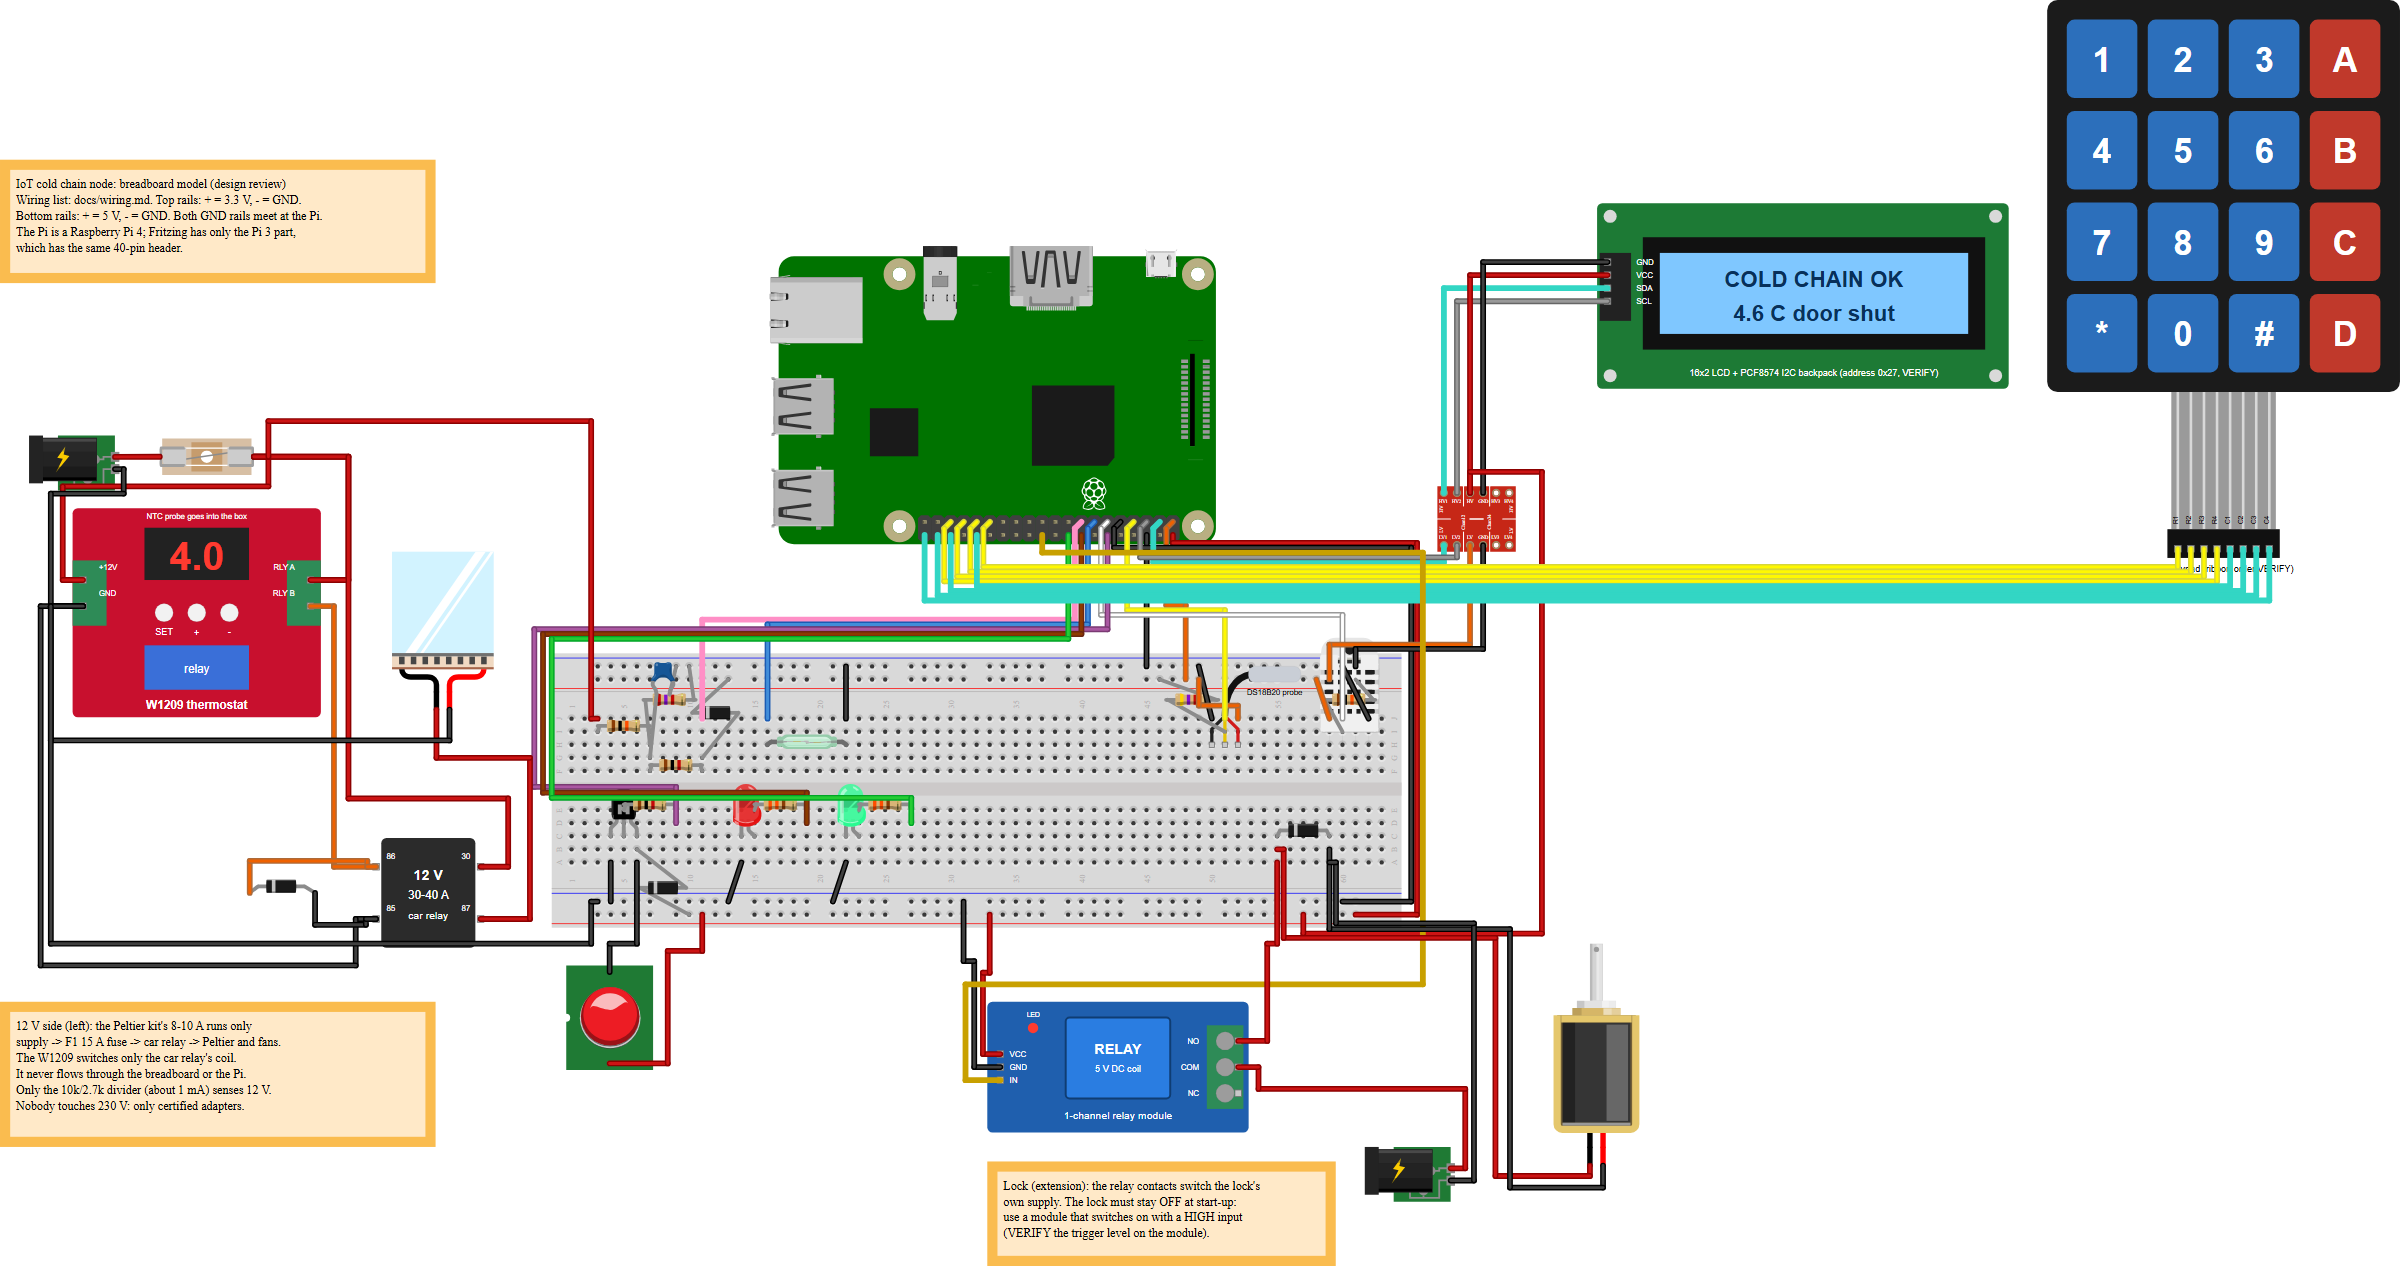
\includegraphics[width=\textwidth]{figures/fritzing-breadboard.png}
\caption{Fritzing breadboard model of the reduced version. Left: 12~V supply, fuse, W1209
thermostat, car relay and Peltier (never on the breadboard). Centre: Raspberry Pi and breadboard with the
sensors, LEDs and buzzer driver. Right: level shifter, LCD and keypad. Bottom: relay module, lock
supply and solenoid lock.}
\label{fig:fritzing}
\end{figure*}

\begin{figure}[!t]
\centering
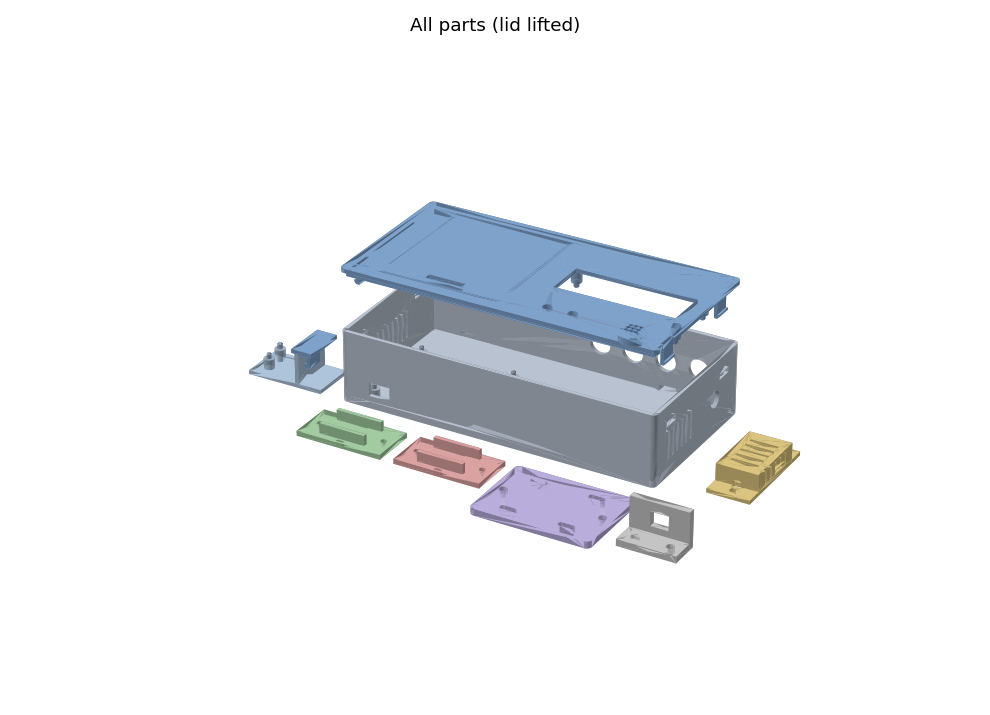
\includegraphics[width=0.49\columnwidth]{figures/enclosure.png}\hfill
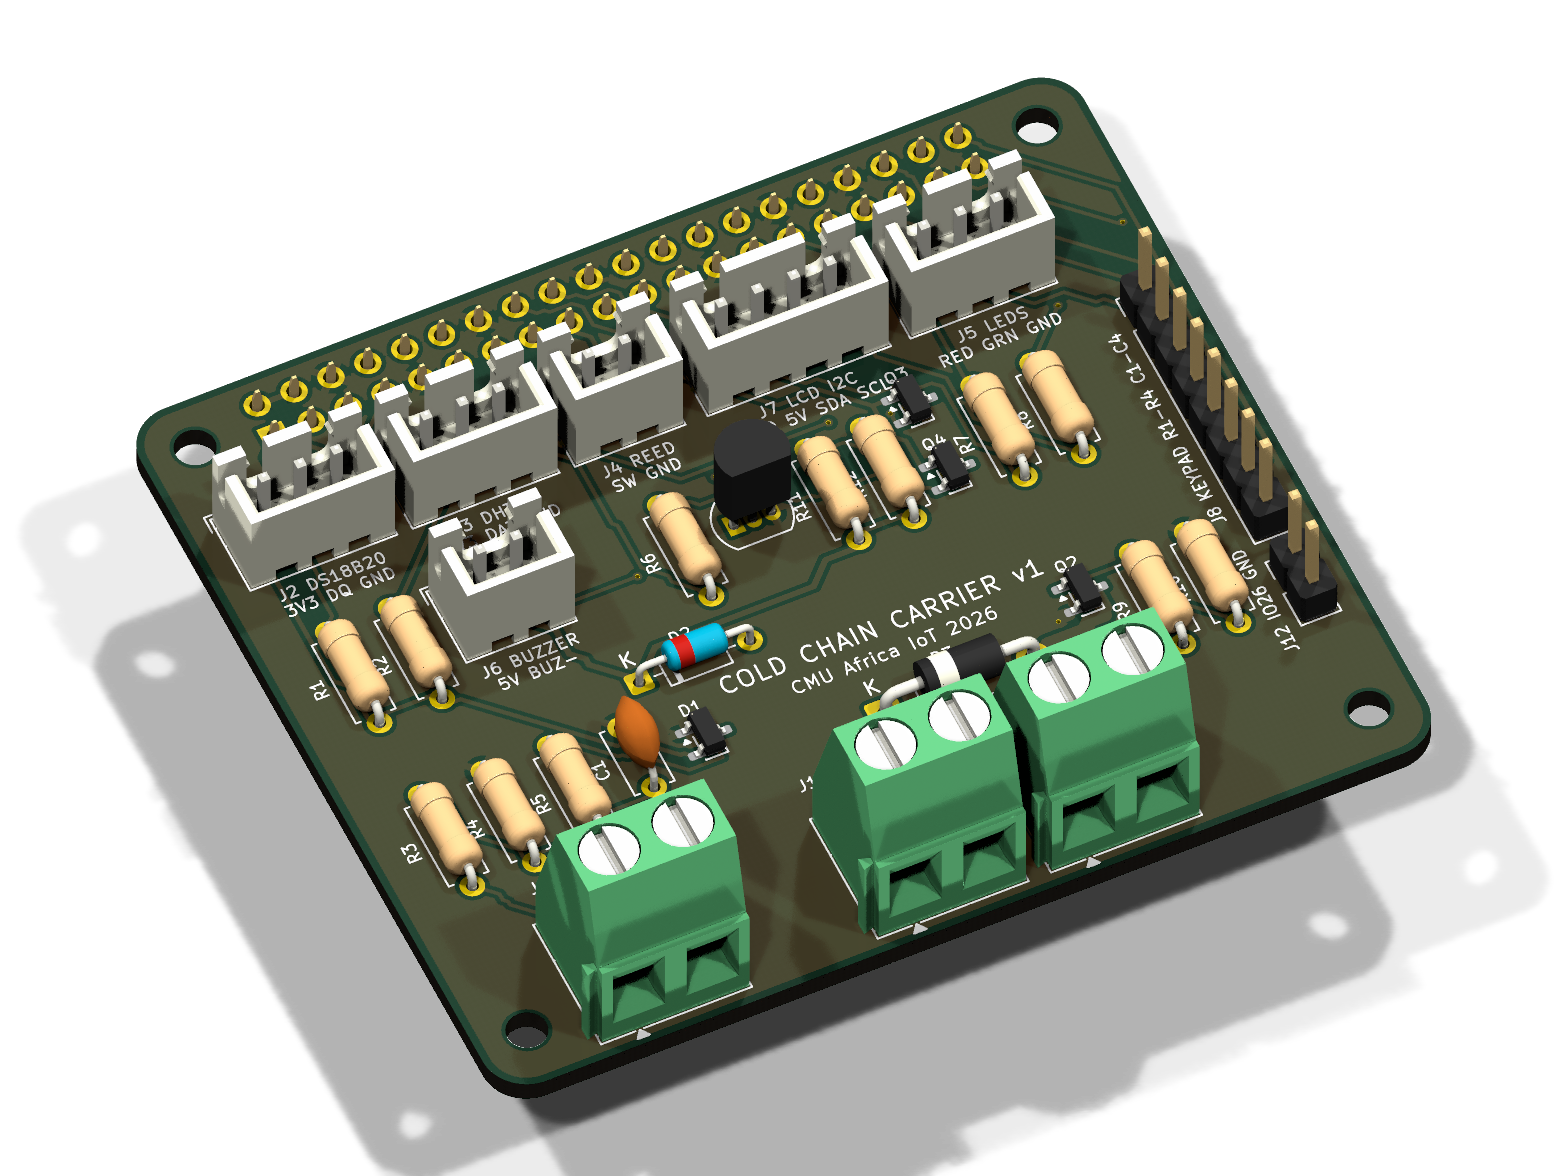
\includegraphics[width=0.49\columnwidth]{figures/pcb-3d.png}
\caption{Left: 3D-printed enclosure (box, lid and sensor holders), designed in FreeCAD. Right:
carrier board for the Pi, designed in KiCad.}
\label{fig:mech}
\end{figure}

\subsection{Firmware of the Edge Node}

The node reads the sensors about every 2~s and feeds a state machine with three states: OK,
WARNING and ALARM. A condition first gives a WARNING; it becomes an ALARM only if it lasts longer
than a confirmation delay, so taking stock out of the fridge does not raise an alarm. The delays
are 300~s for temperature, 120~s for the door and 5~s for power; a demonstration profile uses 20,
15 and 3~s. A 0.3\degC{} hysteresis stops the alarm from flickering at the limit.

The out-of-range timer counts every second outside 2--8\degC{} from the first bad reading, even
before the alarm is confirmed. The total is saved to the SD card every 10~s and at every change,
so it survives a restart. Three bad probe readings in a row raise a sensor fault, and a faulty
value is never counted as time out of range.

The Pi has no real-time clock. It gets the time from the network, and each message carries a flag
saying whether the clock was synchronised. If the node starts without network, it keeps its
messages and corrects their time stamps once the clock is synchronised. The same program also
handles the keypad: PINs are stored as salted hashes, and three wrong PINs lock the keypad for
60~s.

\section{Implementation}

Table~\ref{tab:progress} shows the work breakdown from our proposal, split into smaller tasks, with
the status of each. The software is complete and tested without hardware: 154 unit tests and an
end-to-end test of 34 checks pass. The end-to-end test runs a broker, the back end and a simulated
node together. The back end and the dashboard are deployed on Railway and work with the simulated
node through EMQX: an alarm reaches the dashboard, Firestore and the supervisors' Telegram within
seconds, and the Acknowledge and unlock commands from the dashboard reach the node and are logged
with the supervisor's name. The main open work is the hardware, which depends on the parts we are
buying.

\begin{table}[!t]
\caption{Work breakdown and progress (20 November 2026)}
\label{tab:progress}
\centering
\footnotesize
\renewcommand{\arraystretch}{1.1}
\begin{tabular}{@{}p{3.6cm}p{0.95cm}p{1.75cm}@{}}
\toprule
\textbf{Task} & \textbf{Lead} & \textbf{Status} \\
\midrule
Proposal & Both & Completed \\
Component sourcing & Both & In Progress \\
Fritzing wiring model & Yves & Completed \\
Breadboard wiring & Yves & In Progress \\
Edge firmware and drivers & Yves & Completed \\
Back end, TD and database & Putshu & Completed \\
Design review report & Both & Completed \\
Alarm logic and out-of-range timer & Yves & Completed \\
Dashboard & Putshu & Completed \\
SMS and Telegram alerts & Putshu & Completed \\
Cloud deployment & Putshu & Completed \\
Extension: keypad, lock, QR page & Both & In Progress \\
Enclosure and carrier board & Both & In Progress \\
Integration and testing & Both & In Progress \\
Demonstration & Both & Yet to start \\
Final report & Both & Yet to start \\
\bottomrule
\end{tabular}
\end{table}

\note{Check each status before submitting. ``Breadboard wiring'' is marked In Progress: change it to
Yet to start if you have not wired anything yet. ``Component sourcing'' stays In Progress until the
school's order arrives.}

\section{Discussion}
\label{sec:discussion}

Most of the risk is now in the hardware. The key challenges are:

\begin{itemize}
\item \emph{Parts.} The only Peltier kit sold in Kigali is a 120~W kit that draws about 8--10~A,
almost twice what we planned. We therefore moved to a 30~A supply, a 15~A fuse and a car relay.
No logic-level MOSFET is sold locally, so a relay module switches the lock. Many relay modules
switch on when their input is low; such a module would open the lock while the Pi starts. We must
check the module and use one that switches on with a high input.
\item \emph{Cooling.} We do not yet know how well the kit holds a cool box below 8\degC{} in a
warm room. Frozen gel packs are our fallback for the demonstration.
\item \emph{Power cuts.} In our demonstration, unplugging the 12~V supply stands for a power cut.
In a real cut, the Pi would also lose power unless it has a backup supply. We still need to choose
a UPS board that does not use our GPIO pins.
\item \emph{Cloud services.} The free HiveMQ plan we planned to use closed, so we moved to EMQX
Cloud. The back end and the dashboard now run on Railway.
\item \emph{SMS delivery.} With Africa's Talking's shared sender ID, our messages were accepted
but most were then rejected by the mobile network before reaching our two MTN phones. A registered
sender ID would likely fix this but is expensive, so we added a Telegram bot as a free second
channel: every alert and follow-up goes to both, and a failure on one never stops the other. We
will also ask Africa's Talking why the messages are rejected.
\item \emph{SMS needs the Internet.} The SMS leaves from the cloud, so a site without Internet gets
the local alarm but no SMS. A GSM module on the node would solve this; it is future work.
\end{itemize}

\section{Conclusions}

The design is complete and the software is working. The node, the back end and the dashboard pass
their tests together with a simulated fridge, and the Fritzing model fixes the wiring of the
reduced version. The next steps are to wire the prototype when the parts arrive, measure the
values we marked for checking (the LCD address, the lock current and the divider voltage), print
the enclosure, and rehearse the demonstration of 2 December with the deployed cloud services.

\note{The code is on GitHub, shared with the TA. The report contains no code, as the manual asks.}

\balance

\begin{thebibliography}{3}

\bibitem{who2006}
World Health Organization, ``Temperature sensitivity of vaccines,'' WHO, Geneva, Switzerland,
Rep. WHO/IVB/06.10, 2006.

\bibitem{wot-td}
World Wide Web Consortium, ``Web of Things (WoT) Thing Description 1.1,'' W3C Recommendation,
Dec. 2023. [Online]. Available: \url{https://www.w3.org/TR/wot-thing-description11/}

\bibitem{mqtt5}
A. Banks, E. Briggs, K. Borgendale, and R. Gupta, Eds., ``MQTT Version 5.0,'' OASIS Standard,
Mar. 2019. [Online]. Available:
\url{https://docs.oasis-open.org/mqtt/mqtt/v5.0/mqtt-v5.0.html}

\end{thebibliography}

\end{document}
